\chapter{Model}
\label{model}
\thispagestyle{empty}

In this chapter we describe the derivation of our proposed model. We give again the original formulation of GAN for completeness and then proceed with the related work that lay the necessary steps to our model. We indicate the conditions and assumptions necessary for the model and end with several research questions that we address in chapter \ref{appendiceB} through empirical results.

\section{From GAN to RS}
\label{from_gan_to_rs}
Generative Adversarial Networks \cite{goodfellow2014generative} are now ubiquitous in the Computer Vision domain due to their generative modeling abilities. GANs learn implicitly a probability distribution by being able to generate samples in the data space from a noise input $\textbf{z}$ sampled from a predefined distribution $p(\textbf{z})$. As introduced in \ref{appendiceA}, GANs are composed of two players, usually two neural networks that play a \emph{minimax} zero-sum game in order to learn a target distribution. The objective function that these two networks optimize as given by \cite{goodfellow2014generative} is shown below:
\[
    \min_{G} \max_{D} \E_{x\sim{p_{data}(x)}} [log \, D(x)] + \E_{z\sim{p_{\boldsymbol{z}}(z)}} [log(1-D(G(z)))]
\]
where the discriminator \emph{D} is a binary classifier with the well-known \emph{sigmoid} activation function:
\[
    D(x) = \frac{1}{1 + \exp(-x)}
\]
and the generator G is any neural network that maps noise input $z$ to the data space. As indicated in \ref{appendiceA} the generator network uses the gradient from the discriminator to update its weights and generate better samples to fool the discriminator. In Computer Vision the generator is usually tasked with producing complete images where each composing pixel of the image can take continuous values ranging from 0 to 255.

IRGAN \cite{wang2017irgan} was first to propose the application of GAN for information retrieval and RS. Differently from the original formulation, IRGAN uses the generator network to generate/select item $d$ (e.g. item ID) from a pool of items as the most relevant for a specific user. This generation process is different from applications of GANs in Computer vision because picking items consists in a \emph{discrete} sampling procedure. The objective function in IRGAN (in the context of information retrieval) is given as:
\[
    \begin{split}
        J^{G^*,D^*} = \min_{G} \max_{D} \sum_{n=1}^N(
        & \E_{d \sim{p_{true}(d|q_{n},r)}}[log \, D(d|q_{n})] \: + \: \\
        & \E_{d \sim p_{\theta}(d|q_{n},r)}[log(1-D(d|q_{n}))])
    \end{split}
\]
where $q_{n}$ is a submitted query, $r$ is the relevance distribution of a user over items and $p_{\theta}(d|q_{n},r)$ is the generative model G characterized by parameters $\theta$ that learns to select document $d$ that are most relevant for the submitted query. Since the generator samples discrete values its update cannot be done through gradient descent so for this reason IRGAN uses the policy-gradient based reinforcement learning \cite{williams1992simple}.

CFGAN \cite{chae2018cfgan} brings forward a potential issue in the optimization problem of the discriminator of IRGAN. The aim of the algorithm is for the generator to be able to sample items that are most likely relevant for the user. Consider the beginning of the training procedure of IRGAN. Initially the discriminator has to differentiate between real item IDs and fake item IDs selected by the generator. This is easy in the beginning since the generator is not yet optimal so it will generate IDs that the discriminator can easily detect as not being relevant for the user. However, when approaching the optimality of the generator, the discriminator will be presented with item IDs that are identical to the ones already in the historical profile of the user but are presented to the discriminator labelled as \emph{real} (when the item ID is coming from the real training data) and \emph{fake} (when the item ID is coming from the generator) at the same time. CFGAN empirically shows that training IRGAN up to this point confuses the discriminator and deteriorates the accuracy of the algorithm.

\begin{figure}[htbp]
    \centering
    \begin{subfigure}[b]{0.48\textwidth}
        \centering
        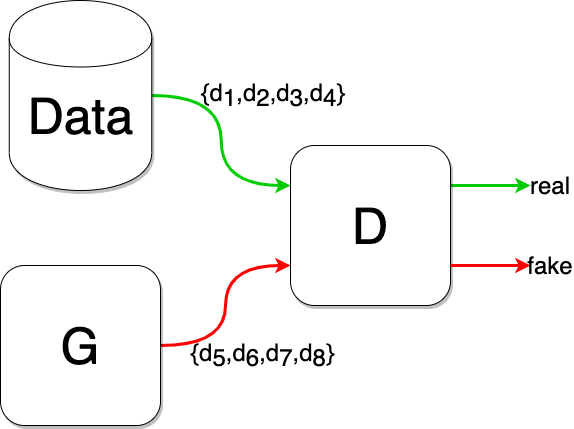
\includegraphics[width=\textwidth]{model/irgan_problem1.png}
        \caption{IRGAN model in the first epochs of training. The items picked by the generator are different from the ground truth.}
        \label{fig:irgan_problem1}
    \end{subfigure}
    \hfill
    \begin{subfigure}[b]{0.48\textwidth}
        \centering
        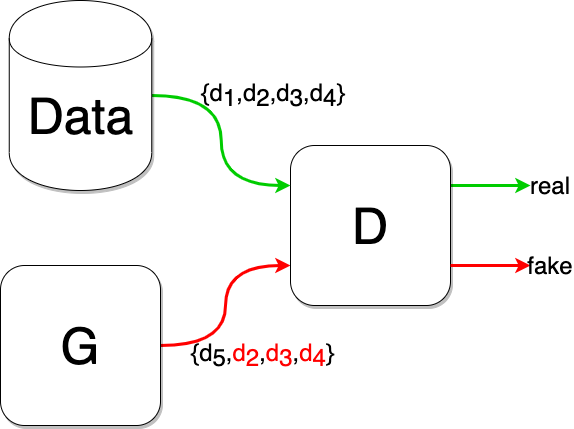
\includegraphics[width=\textwidth]{model/irgan_problem2.png}
        \caption{IRGAN model near/at optimal generator. The generator picks items with the label \emph{fake} identical to those in the training set which the discriminator has seen as \emph{real}.}
        \label{fig:irgan_problem2}
    \end{subfigure}
    \caption{Discrete item generation issue with IRGAN.}
    \label{fig:irgan_problem}
\end{figure}

To solve this problem CFGAN proposes a vector-wise training for RS where the generator G outputs \emph{real-valued} vectors. In this way D can discriminate between real user historical interactions and plausible historical interactions produced by G.

\section{GANMF}
\label{sec:GANMF}
Our model, which we denote as GANMF, attemps to solve the generic Top-N recommendation problem presented in \ref{appendiceA}. We take a model-based approach for the recommendations and structure GANMF as a matrix factorization model. We task our model to learn the distribution of historical interactions of each respective user utilizing the \emph{vector-training} introduced by CFGAN. This means for the generator to be able to produce historical profiles that are very similar to the training data but differ in such a way that can provide recommendations better than (comparable to) other MF-based baselines. GANMF follows the original GAN formulation and is composed of two players, a generator network G and a discriminator network D. GAN allow the modeling of \emph{multi-modal} outputs \cite{goodfellow2016nips} where for a specific input there might be multiple correct outputs or labels. For this reason the input of the generator in a GAN is usually some noise from a predefined distribution. By using this noise GANs can produce diverse samples that resemble the training data. However, in our case the recommendation must be deterministic and unique in order for it to provide the best user experience and make it feel personalized for the users. This urges the conditioning of the generation process on each user available in our training data.

\subsection{Discriminator D}
\label{sec:GANMF_D}
The discriminator in a GAN is used to differentiate the source of the data it takes as input. As mentioned in \ref{from_gan_to_rs} the discriminator is usually a binary classifier and in the original formulation it outputs the probability of the input being real and not generated by G. For GANMF we take another approach and model D according to the discriminator in EBGAN \cite{zhao2016energy}. As described in \ref{appendiceA}, EBGAN was first to introduce the discriminator as an energy function where is assigns low energy to samples in the data manifold and high energy elsewhere. In this context we can think of the energy function as a hyperplane which takes the shape of a valley near real data that come from the training set and takes the shape of mountains near data generated by G. Just like EBGAN, GANMF uses an autoencoder \cite{kramer1991nonlinear} as the discriminator where the reconstruction loss acts as the energy function:
\begin{equation}
    D(x) = ||Dec(Enc(x)) - x||
    \label{eq:recon_loss}
\end{equation}
where $Enc(\cdot)$ and $Dec(\cdot)$ are the \emph{encoder} and \emph{decoder} functions and $||\cdot||$ is the Euclidean norm.

The rationale for using an autoencoder model as discriminator falls in the same line of the discussion by the authors of EBGAN. In the original formulation the discriminator's output is a scalar value squashed in the range $[0-1]$ by a \emph{sigmoid} activation indicating a probability. The output of the generator in the case of GANMF is very high dimensional; specifically it is the length of a user historical profile $|I|$, which for some datasets might be in thousands or even millions of dimensions. Updating the weights of the generator through the gradient of a single scalar value in the discriminator output poses difficulties for learning the generator. Consider the case when two generated historical profiles for the same user, $\hat{I^1_{u}}$ and $\hat{I^2_{u}}$, differ between each other a lot but for the discriminator they are both fake profiles. The gradient propagated back to update the weights is going to be more or less the same for both generated profiles. Assuming $I^*_{u}$ to be the optimal generated profile for user $u$ then under some distance metric (e.g. Euclidean distance) we have:
\[
||I^*_{u} - \hat{I^1_{u}}|| \leq  ||I^*_{u} - \hat{I^2_{u}}||\quad \bigvee \quad
||I^*_{u} - \hat{I^2_{u}}|| \leq  ||I^*_{u} - \hat{I^1_{u}}||
\]
yet the gradient coming from the discriminator will not make this distinction very clear. Also when training through Mini Batch Gradient Descent, having a single value output makes the gradient for the batch highly unlikely to be orthogonal for the individual batch samples \cite{zhao2016energy}. We further explore the effect of the autoencoder as the discriminator through experiments.

Given a real data $x$ and a user conditioning vector $y$ (more on this in \ref{sec:GANMF_G}) the loss function for GANMF discriminator is given by the \emph{hinge loss} \cite{zhao2016energy}:
\begin{equation}
    \mathcal{L}_{D}(x, y) = D(x) + [m - D(G(y))]^+
    \label{eq:dloss}
\end{equation}
where $[\cdot]^+ = \max (0, \cdot)$, $m$ is a positive margin, $D(\cdot)$ is the autoencoder reconstruction loss as defined in (\ref{eq:recon_loss}) and $G(\cdot)$ is the generator function.
D (the discriminator, not the $D(\cdot)$ function) is trained to minimize \ref{eq:dloss}. The first term denotes the reconstruction error of the autoencoder on real user profiles. Since the reconstruction error is always positive the minimum of this term is 0 meaning a perfect reconstruction. The second term involving the $\max$ operator can be summarized as:
\[
    [m - D(G(y))]^+ = \max (0, D(G(y))) = 
    \begin{cases}
        0 & D(G(y)) \geq m \\
        m - D(G(y)) & D(G(y)) < m
    \end{cases}
\]
This term tries to keep the reconstruction loss of generated user profiles above the margin value. Since the discriminator is trying to minimize this term also, the autoencoder's weights are updated in such a way as to prevent the reconstruction error falling below the margin otherwise it is penalized by how much the error violates it. If the reconstruction loss is more than the margin, the second term reaches its minimum at 0. Using the $\max$ operator we achieve a higher energy value for the generated user profiles. This operator is common in training Support Vector Machines where optimal class-separating hyperplane is the one that does not violate the margin from the support vectors \cite{cortes1995support}. In GANMF $m$ is a hyperparameter of the model which we tune through a hold-out validation set.

\subsection{Generator G}
\label{sec:GANMF_G}
We now detail the generator network. As stated in section \ref{sec:GANMF}, we construct G as a conditional generator by using as condition attributes that are unique to each user. These attributes serve as the only input to a fully-connected neural network. In \cite{strub2016hybrid} the authors show that a single layer autoencoder with linear activation function in the output layer is very similar to a low-rank MF approach. Following this observation, we use only one hidden layer for the generator. This is an embedding layer that takes the user conditioning vector as input and constructs a representation out of it. We set the dimension of this layer to the number of latent factors for our MF-based model. Since the conditioning vector will be deterministic and unique for each user, the output of the hidden layer will act as a representation of the user, namely his/her latent factors. The output layer of the generator will have the same dimension as the length of a user historical profile, $|I|$. 

Let us consider a single-layer fully-connected neural network (see figure \ref{fig:generator_MF}). The first layer $l^0$ represents the input, the user conditioning vector in the GANMF case. The nodes in this layer are all connected to the nodes in the hidden layer $l^1$ which represents the user latent factors. The output of this hidden layer is:
\[
l^1_{j \in nodes(l^1)} = h(\sum_{i \in nodes(l^0)} W^0_{ji} \; l^0_{i})
\]
where $h(\cdot)$ is the activation function of the hidden layer and $W^0$ is a weight matrix of shape $|ConditionVector| \times K$ (we omit the bias term). The same stands for layers $l^1$ and $l^2$ where the latter is the output of the network denoting a generated user profile.
\begin{equation}
l^2_{k \in nodes(l^2)} = g(\sum_{j \in nodes(l^1)} W^1_{kj} \; l^1_{j})
\label{eq:output_layer_mult}
\end{equation}
where $g(\cdot)$ is the linear activation function for the output layer and $W^1$ is the weight matrix of shape $K \times |I|$ (we omit the bias term).
\begin{figure}[h!]
    \centering
    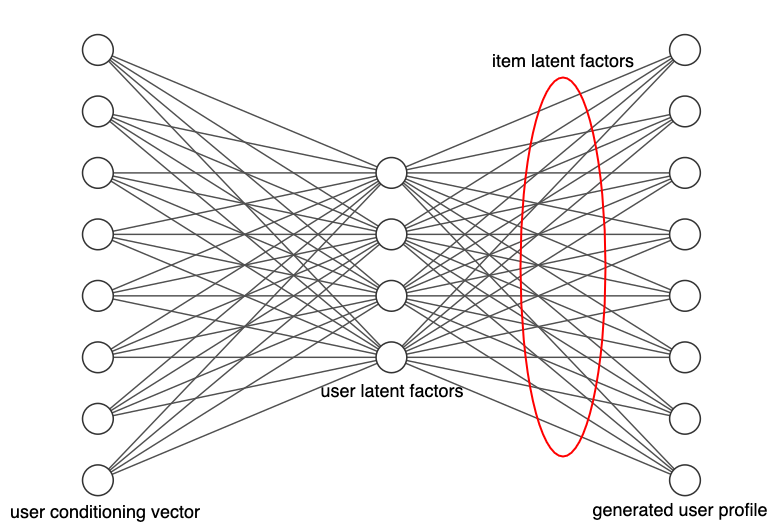
\includegraphics[width=0.95\textwidth]{model/fully_connected_generator.png}
    \caption{GANMF Generator representing a low-rank MF model. The edges connecting the per-user latent factors to the output layer represent the items latent factors.}
    \label{fig:generator_MF}
\end{figure}

Low-rank MF model aim to factorize a rectangular matrix into two low-rank matrices (in a RS context):
\[
\begin{split}
    \hat{URM} & = \Sigma V \\
    \hat{URM} & \in \mathbb{R}^{|U| \times |I|} \\
    \Sigma & \in \mathbb{R}^{|U| \times K} \\
    V & \in \mathbb{R}^{K \times |I|} \\
    K & \ll |U| \\
    K & \ll |I|
\end{split}
\]
where $\Sigma$ and $V$ are the users' and items' latent factors' matrices respectively and $\hat{URM}$ is an approximation of the URM from which we derive the recommendations for users. We can retrieve a users' predicted profile by selecting a row from $\hat{URM}$ which in itself can be retrieved by:
\begin{equation}
    \hat{URM_{u}} = \Sigma_{u}V
    \label{eq:mf_vector_matrix}
\end{equation}
$\Sigma_{u}$ is the row-vector of size $K$ corresponding to the same row in $\hat{URM}$. One can observe that equation \ref{eq:output_layer_mult} denotes the same vector-matrix multiplication operation as \ref{eq:mf_vector_matrix}.

\begin{figure}[h!]
    \centering
    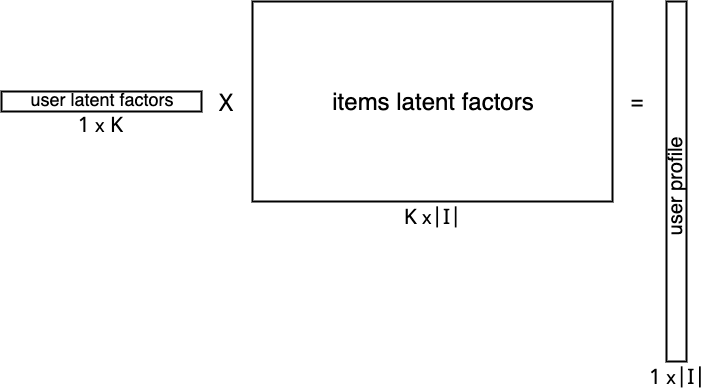
\includegraphics[width=0.95\textwidth]{model/vector-matrix.png}
    \caption{The low-rank matrix factorization model derived from a fully connected neural network.}
    \label{fig:vector_matrix}
\end{figure}

Since we are utilizing only the URM, we are limited to two options in regards to possible conditioning vectors; we can either use the row number in the URM respective to the user or the complete URM row-vector that represents the historical profile of the user. In the former case the generator input is just an integer value in the range $[1-|U|]$. The neural network framework we used to implement GANMF provides a convenient \emph{embedding} layer that performs a table lookup of embedding values from integer values. These embeddings are task-specific and are learned in conjunction with the whole network. A clear advantage of this option is that the number of parameters to be learned by the generator is $\Theta(K\times(|I|+|U|))$, similar to baselines like ALSMF. 

If we choose to use the complete row-vector from the URM of a specific user as conditioning vector, the input dimension of the generator would be $|I|$, just like the output layer dimension. In this case the generator takes the role of an autoencoder and we can use the same arguments to show that this network also can be casted into a low-rank MF approach. We conduct experiments with both of these options in order to understand whether a more detailed historical information can produce better user latent factors.

The generator's job is to fool the discriminator of GANMF. While the discriminator's job is to increase the reconstruction loss of generated user profiles, the generator tries to minimize the reconstruction loss:
\begin{equation}
    \mathcal{L}_{G}(y) = D(G(y))
\end{equation}
where $G(\cdot)$ and $D(\cdot)$ are the generator and discriminator functions respectively and $y$ is the user conditioning vector.

\subsection{Single-sample class conditioning}
\label{sec:ss_class_conditioning}

As stated in section \ref{sec:GANMF}, GANMF at its core is a conditional GAN (cGAN) of the type presented in \cite{mirza2014conditional}. Usually the condition input in a cGAN is a label or class associated with the data sample passed to the generator in order to condition the generation process but also to the discriminator so it can judge the realness of the data sample given the label. Applications of cGAN usually involve datasets with multiple classes where for each single class there are hundreds or thousands of samples from the training set. This allows the discriminator to learn not only the source of the samples it receives but also a relation between the sample and its label.

We experimented with a binary classifier discriminator (as per the original formulation of GAN) where the input was the concatenation of a real/generated profile with the conditioning vector representing the user of the profile. We faced a peculiar problem with this version of GANMF; the user latent factor resulting from the training where very similar with one another and the quality (see evaluations) of the recommendations was very poor. However, considering that for every single user we only have one real historical profile this finding is not a surprise. Generalizing the variable-label relation from a single data point per label is almost impossible.

To alleviate this problem and further improve the accuracy of the recommendations we follow an approach called \emph{feature matching} from \cite{salimans2016improved}. Feature matching is presented as a technique to stabilize the training procedure of GANs and also avoid \emph{mode collapse} (see section \ref{appendiceA}). During training, the generator might trick the discriminator very easily by finding a sample that the discriminator cannot distinguish from the real data and always generate that particular sample or minor variations of it. Usually this single sample need not even be recognizable as a meaningful data point in comparison with the dataset at hand (e.g. if generating images of handwritten digits the output of the generator could be a tower in a black background which might resemble the digit one and hence the reason the discriminator cannot distinguish it but is entirely not related to what we are expecting from the generator). Feature matching changes the objective of the generator to not deceive the discriminator but match real data statistics by using the following loss term:
\[
||\E_{\textbf{x} \sim{p_{data}}} \textbf{f}(\textbf{x}) - \E_{\textbf{z} \sim{p_{z}(\textbf{z})}} \textbf{f}(G(\textbf{z}))||^2_{2}
\]
where $\textbf{f}(\cdot)$ is the activation of an intermediate layer of the discriminator, $G(\cdot)$ is the generator function, and $||\cdot||^2_{2}$ is the Euclidean norm squared.

We incorporate this technique in GANMF as a way to enforce conditioning the generating process. The conditioning vector in GANMF is necessary for the generator in order to retrieve the user latent factors. However, the generating process could still be stuck by discarding the information in the conditioning vector and by finding a specific user profile that deceives the GANMF discriminator (when reconstructed in the discriminator, the loss is the same as the average loss of all real user profiles). To force the generator to learn user-specific latent features we change the previous loss of the generator to the following:
\begin{equation}
    \mathcal{L}_{G}(x, y) = \beta \, D(G(y)) \, + \, (1-\beta) \, || \, l^1(x) - l^1(G(y)) \,||^2_{2}
    \label{eq:generator_loss_feature}
\end{equation}
where $l^1$ is the activation of the hidden layer of the autoencoder (discriminator, see section \ref{sec:GANMF_D}), $D(\cdot)$ and $G(\cdot)$ are the discriminator and generator functions respectively, $x$ and $y$ are a real user profile and the corresponding conditioning vector respectively and $\beta$ is a weighting term that decides the balance of the generator between deceiving the generator and matching the hidden layer activations.

The second term of $\mathcal{L}_{G}$ takes the form of another autoencoder incorporating the generator and the encoder part of the discriminator. Given real user profile $x$ and its corresponding conditioning vector $y$ we first retrieve the hidden layer activation of the discriminator for $x$, $l^1(x)$. Then we generate a plausible user profile for $y$, $G(y)$. We retrieve the hidden layer activation of the discriminator for $G(y)$, $l^1(G(y))$. If the generated profile is indeed suitable for the user denoted by $y$ then we should have that $l^1(x)$ and $l^1(G(y)$ must be close to each other by some distance metric (here we use the Euclidean distance squared as \cite{salimans2016improved}).

\begin{figure}
    \centering
    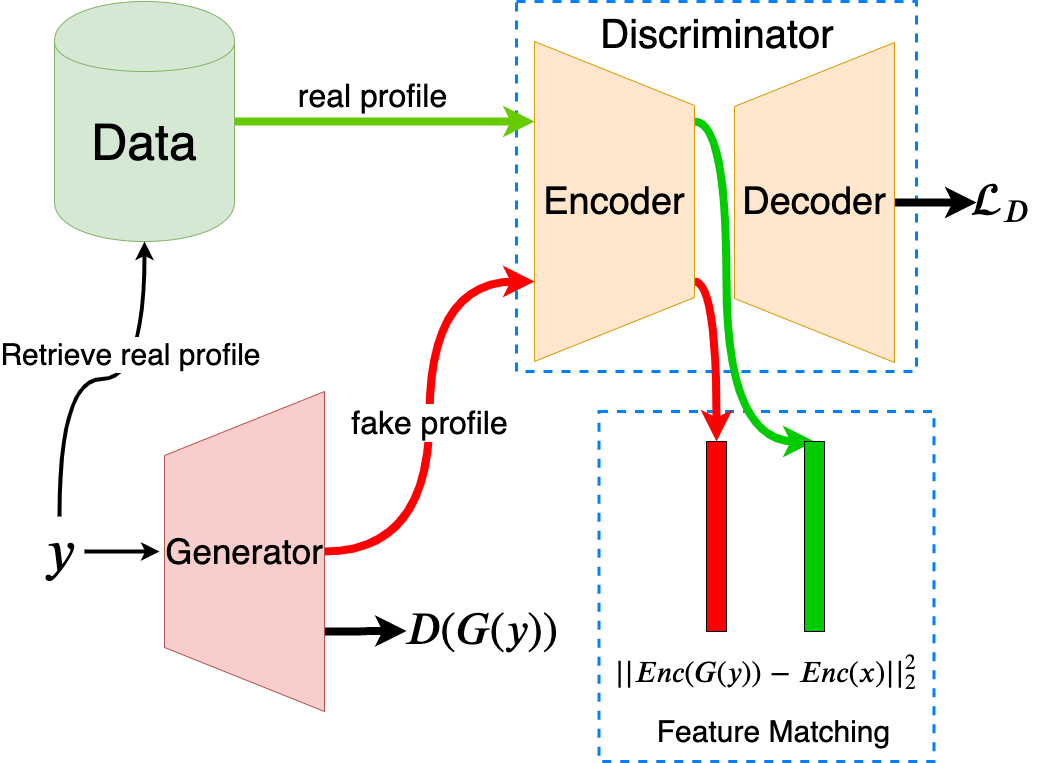
\includegraphics[width=0.95\textwidth]{model/full_GANMF.png}
    \caption{Architecture of GANMF: the conditioning vector $y$ represents the row number of a user in the URM.}
    \label{fig:full_ganmf}
\end{figure}

\subsection{Training}
Figure \ref{fig:full_ganmf} depicts the full GANMF model. Since we are using the vector-training approach from CFGAN, we can bypass the policy-gradient based reinforcement learning used by IRGAN and train the complete model end-to-end by Gradient Descent and Backpropagation \cite{rumelhart1986learning}.